\documentclass[10pt]{beamer}
\usepackage{amsmath}
\usepackage{amssymb}
\usepackage{geometry}
\usepackage{graphicx}
\usepackage{url}
\usepackage{xcolor}

\begin{document}

%---------------------------------------------
\begin{frame}
\large
Lecture 1:\\
Introduction\\
STAT 630, Fall 2021
\end{frame}

%---------------------------------------------
\begin{frame}{Outline of Course Topics}
This course will have four main components:
\vspace{5pt}
\begin{itemize}
\item Data collection: sampling designs and experimental studies
\vspace{5pt}
\item Exploratory data analysis: numerical summaries and graphical displays of data
\vspace{5pt}
\item Statistical inference: hypothesis testing and confidence intervals 
\vspace{5pt}
\item Linear regression and correlation\\
\end{itemize}
\vspace{10pt}
We will also review some probability concepts.  Most of you are enrolled in STAT 620, and will be learning probability theory concurrently. 
\end{frame}

%---------------------------------------------
\begin{frame}{Grading}
There will be weekly homework assignments, and three take-home exams.  Both the homework and exams will be a combination of conceptual and data analysis problems.  The data analysis problems will require the use of R.  Late homework will generally not be accepted.  However, your lowest scoring homework assignments will be dropped.\\
\vspace{5pt}

\begin{itemize}
\item 25\% Homework
\vspace{5pt}
\item 75\% Three Exams (25\% each)
\end{itemize} 
\end{frame}

%---------------------------------------------
\begin{frame}{Textbook}
Diez, D., Barr, C. and Cetinkaya-Rundel M. \emph{OpenIntro: Statistics}, 4th Edition, 2019.\\
\vspace{5pt}
Free PDF version posted on Blackboard in the ``Resources" folder.\\
\vspace{10pt}
This will be the main textbook for the course.  It provides a very accessible and concise introduction to statistics.  It is written at the undergraduate level, but is also popular in graduate courses.  It also includes an R package with many data sets that we will use during lab.  
\begin{figure}
\flushright
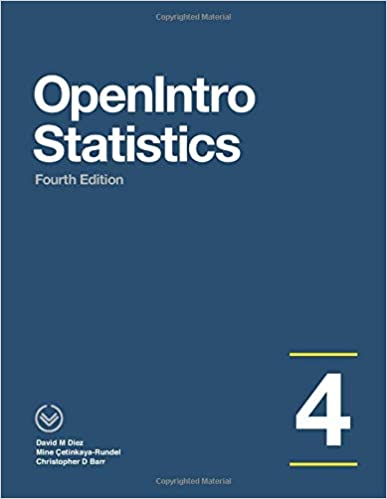
\includegraphics[scale=0.15]{figure/oi_cover.jpg}
\end{figure}
\end{frame}

%---------------------------------------------
\begin{frame}{Textbook}
Chihara, L. and Hesterberg T. \emph{Mathematical Statistics with Resampling and R}. 2nd Edition, 2018.\\
\vspace{5pt}
Free electronic version: \url{http://library.csueastbay.edu/home}\\
\vspace{10pt}
This textbook provides an introduction to mathematical statistics with an emphasis on computational methods for doing statistical inference.  It is written at the advanced undergraduate or first-year graduate school level.  We will reference this book when covering resampling techniques such as the bootstrap.  The book also contains some mathematical derivations not covered in OpenIntro.
\begin{figure}
\flushright
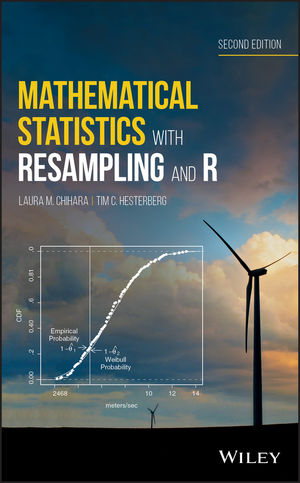
\includegraphics[scale=0.15]{figure/msr_cover.jpg}
\end{figure}
\end{frame}

%---------------------------------------------
\begin{frame}{Labs and Software}
Weekly computer labs will focus on learning the R programming language and using it for statistical data analysis.  Topic we will cover in lab include:\\
\begin{itemize}
\item Vectors and data frames
\item Subsetting data frames
\item Looping and control structures
\item Summarizing data and creating graphics
\item Loading data files into R
\item Simulation and resampling techniques
\item Report writing and reproducible research (R Markdown)\\
\end{itemize}

We will often replace and compare mathematical (analytic) techniques for doing statistics with more flexible and intuitive computational approaches.  
\end{frame}

%---------------------------------------------
\begin{frame}{Why learn R?} 
\begin{itemize}
\item It is a \textbf{free} and open-source software that runs on most operating systems (Windows, Mac, Linux).  
\item It is one of the most \textbf{popular} programming languages used for statistics and data science.  
\item It is a desired and necessary skill for many statistics and data science \textbf{jobs} in academia, industry, and government.
\item It is a legitimate programming language that allows more control and \textbf{reproducibility} than a point-and-click interface. 
\end{itemize}
\begin{figure}
\flushright

\includegraphics[scale=0.2]{figure/Rlogo.png}
\end{figure}
\end{frame}

%---------------------------------------------
\begin{frame}{RStudio}
\begin{itemize}
\item RStudio is a popular interface for using the R programming language.
\vspace{5pt}
\item RStudio provides a code editor, console, and tools for plotting, debugging, and version control.
\end{itemize}
\begin{figure}
%\flushright
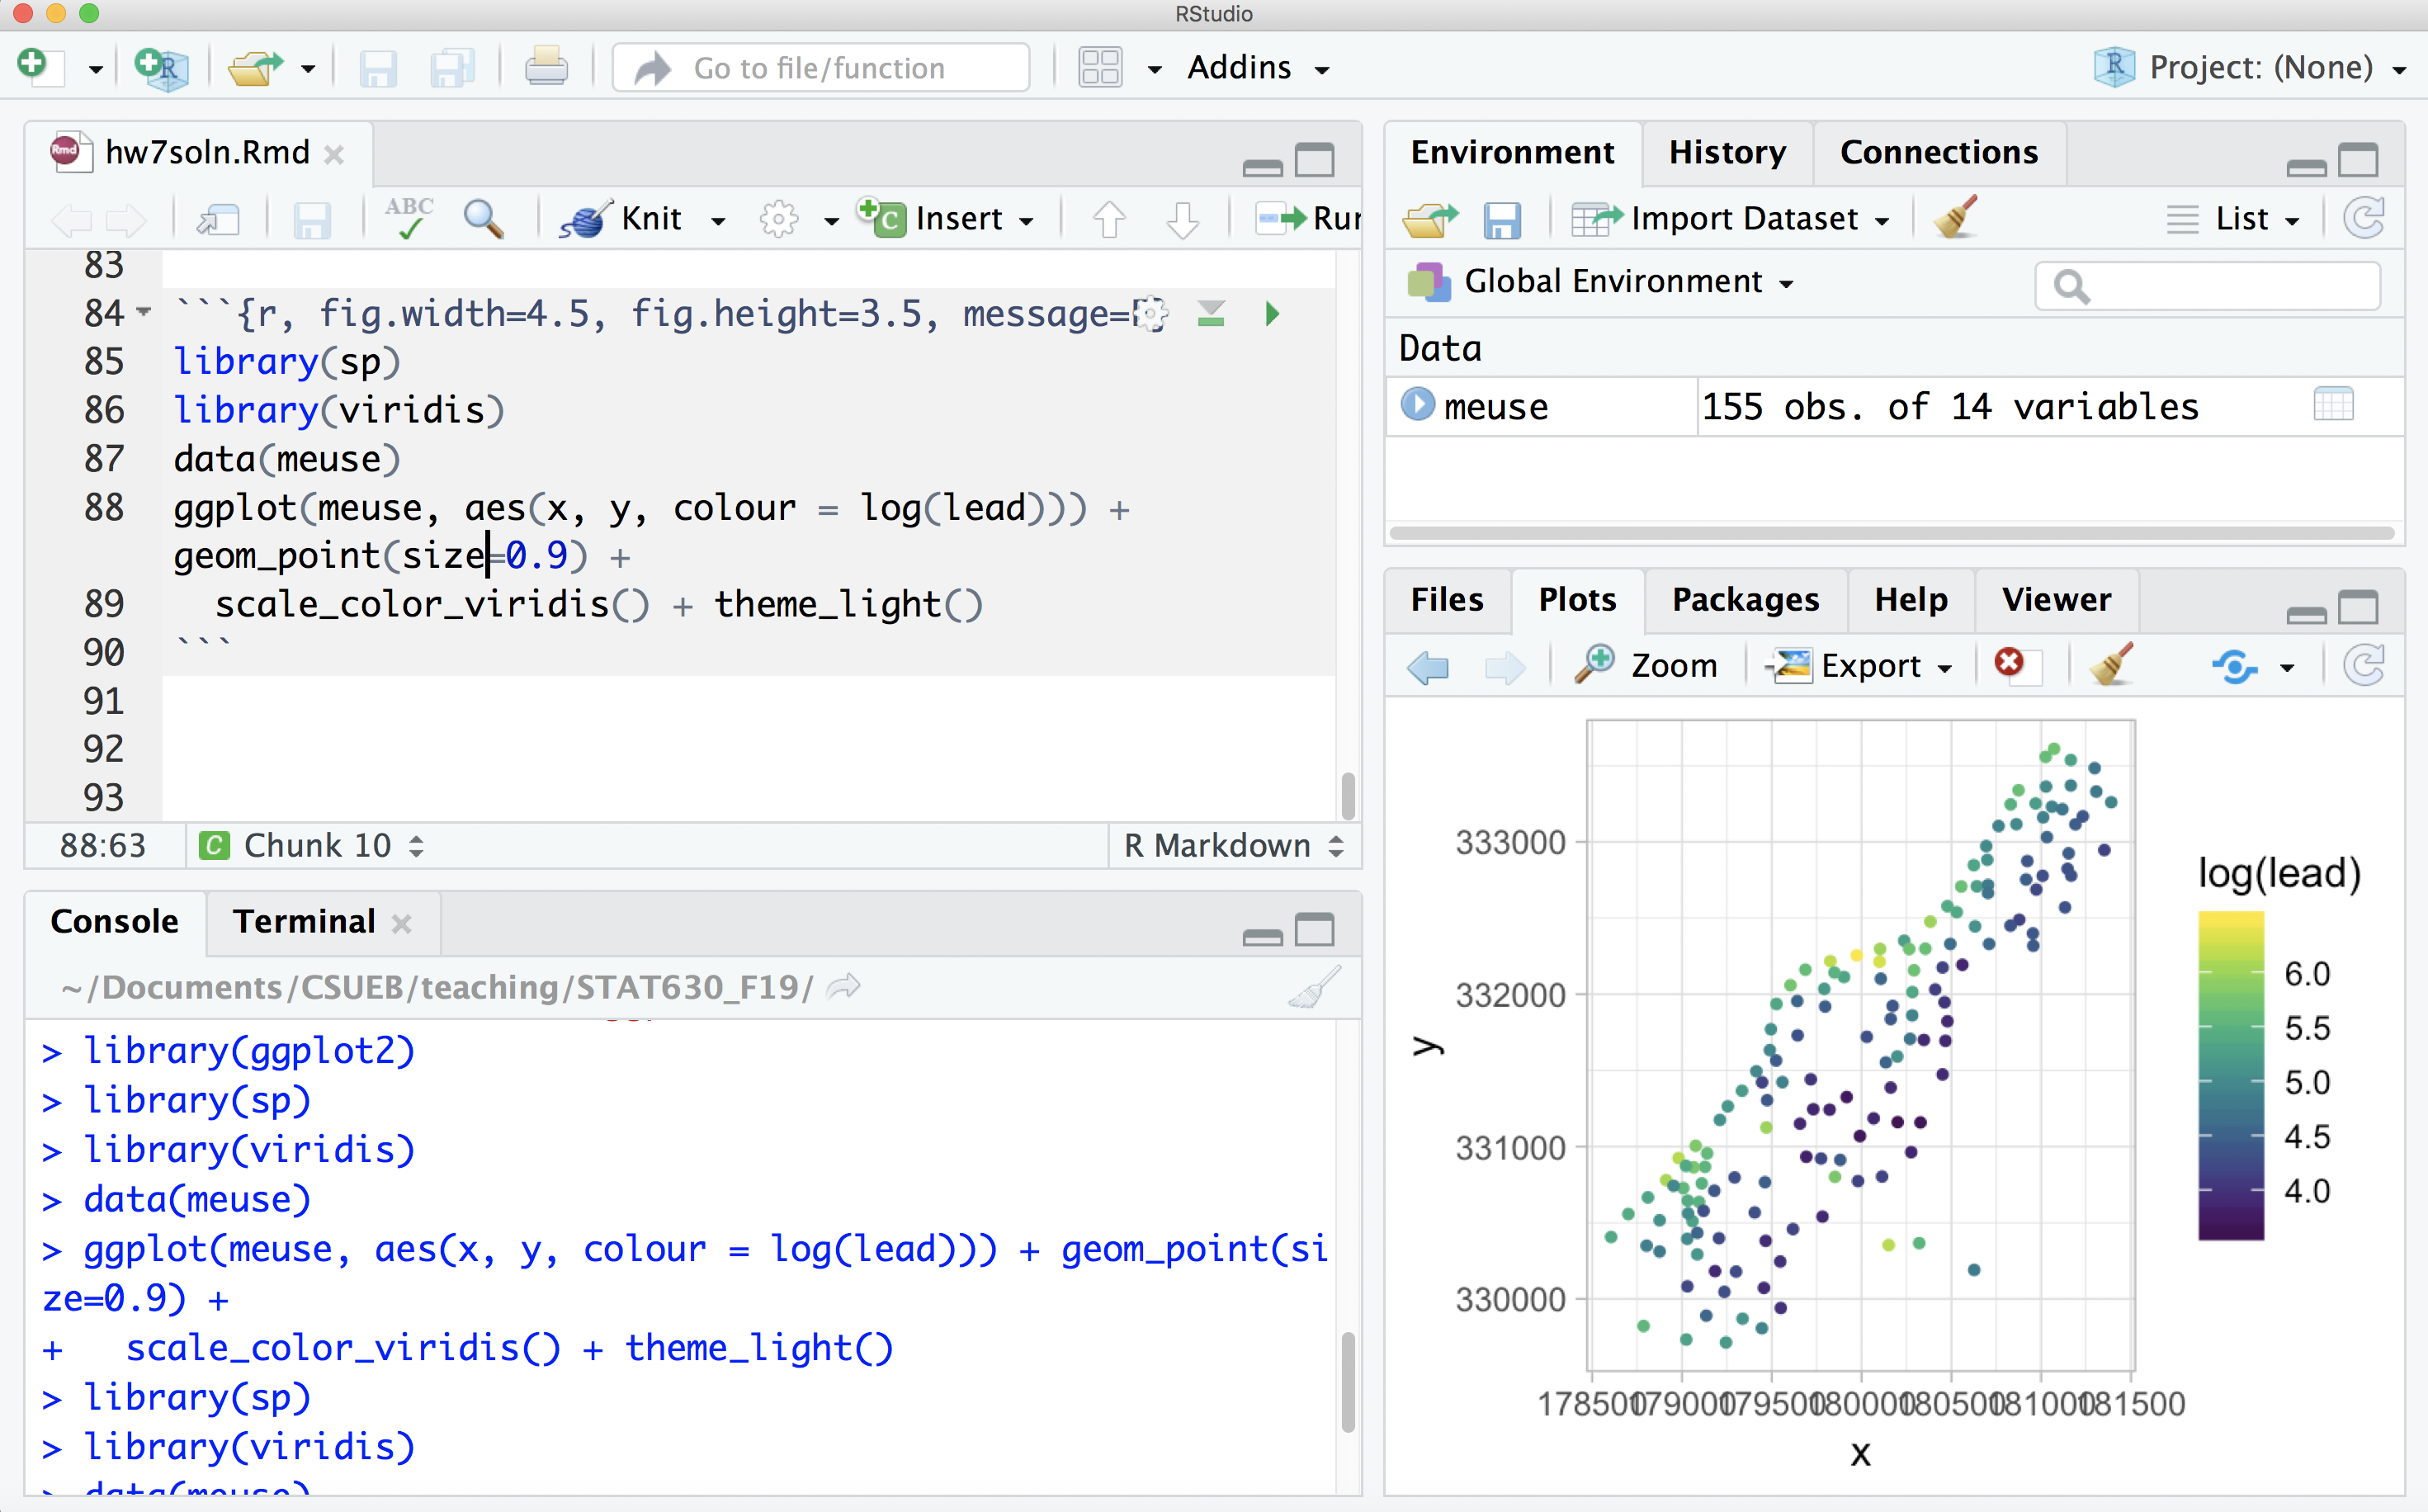
\includegraphics[scale=0.15]{figure/RStudio_screenshot.png}
\end{figure}
\end{frame}

%---------------------------------------------
\begin{frame}
Redmonk rankings of different programming languages based on GitHub repositories (developer activity) and Stack Overflow activity (user discussion forums).
\begin{figure}
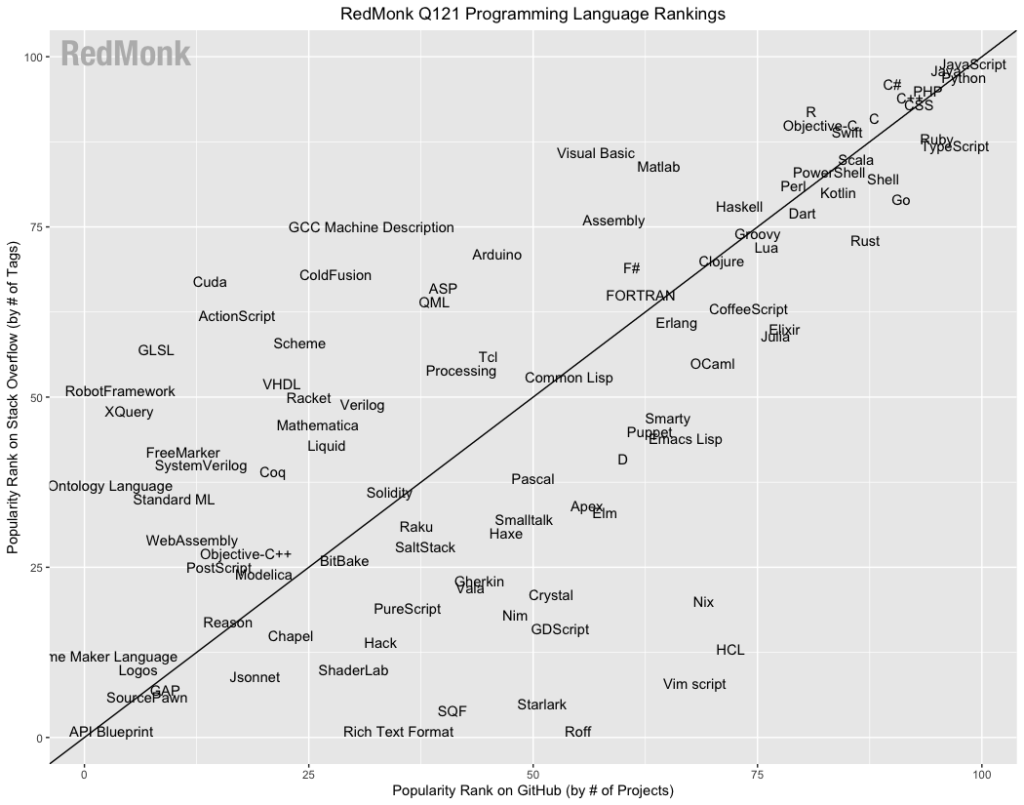
\includegraphics[scale=0.17]{figure/redmonk2021.png}
\end{figure}
\scriptsize Source: \url{https://redmonk.com/sogrady/2021/03/01/language-rankings-1-21/}
\end{frame}
% Above the 80th percentile
% R has been a favorite language amongst statisticians and data scientistis for over a decade.  Although, Python ranks higher since it is a more general purpose computer programming language.

%---------------------------------------------
\begin{frame}{Preliminaries}
The \textbf{field of statistics} is broadly concerned with collecting, analyzing and interpreting data for the purpose of decision making and scientific discovery.
\vspace{15pt}

A statistical investigation often follows these steps:
\begin{enumerate}
\item Define the problem, and formulate research questions
\item Design the sampling procedure or experiment for collecting the data
\item Explore and analyze the data  
\item Formulate conclusions and communicate the results\\
\end{enumerate}
\end{frame}

%---------------------------------------------
\begin{frame}{Preliminaries}
More generally, we can view the steps of a statistical investigation as an iterative process, represented by the ``Data Cycle" shown below.
\begin{figure}
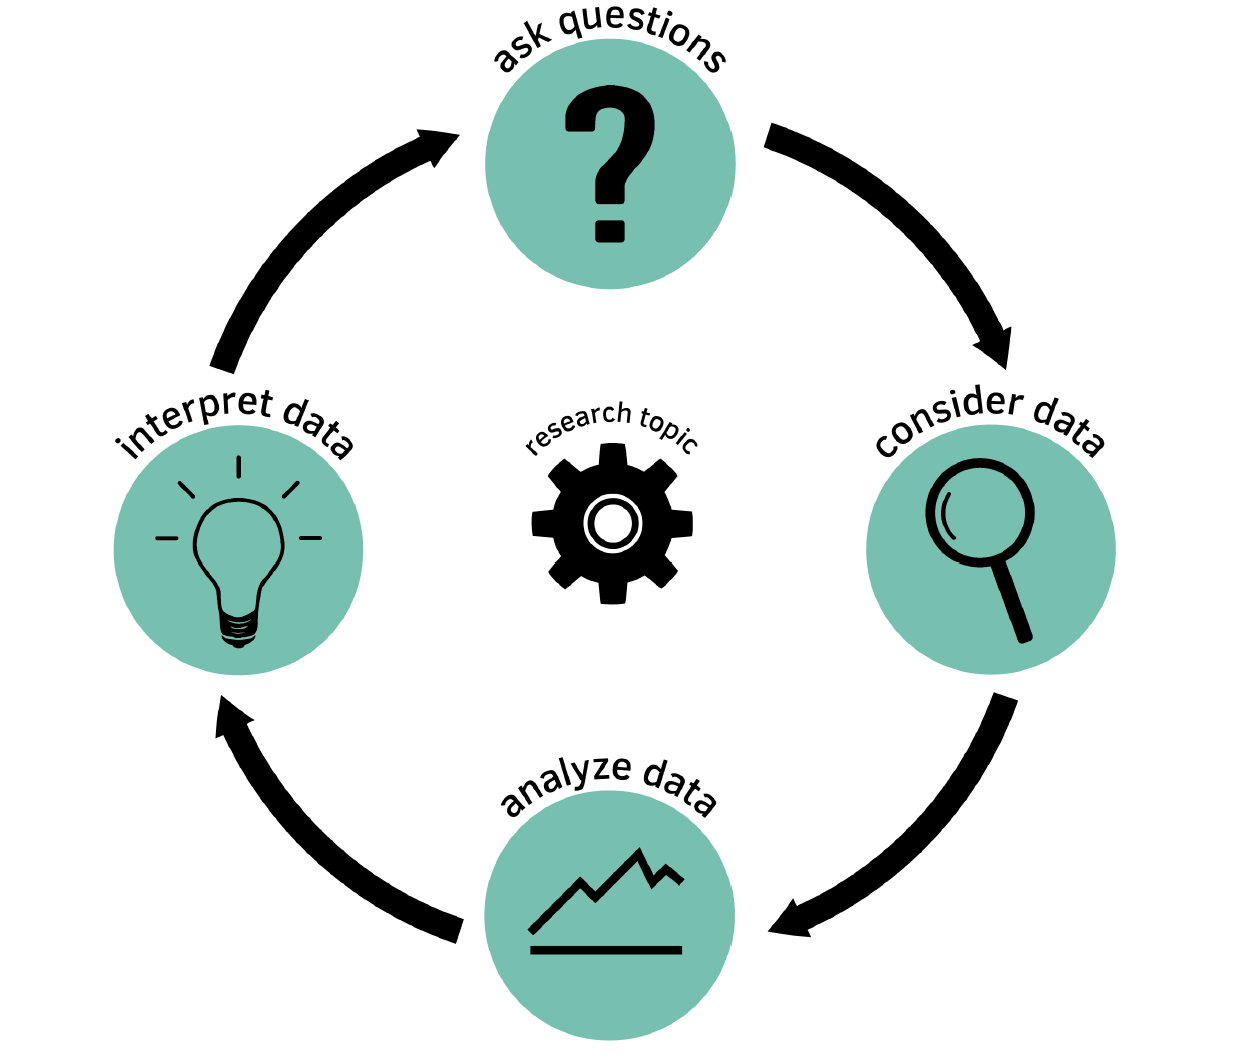
\includegraphics[scale=0.25]{figure/data_cycle.png}
\end{figure}
% The second stage was intentially called "consider" data instead of "collect" data since often the data has already been collected and just needs to be prepared for the analysis
\scriptsize Image from Robert Gould et al. (2016). ``Teaching data science to secondary students: The mobilize introduction to data science curriculum." \url{http://iase-web.org/documents/papers/rt2016/Gould.pdf}
\end{frame}

%---------------------------------------------
\begin{frame}
\large \textbf{Introducing Data}
\begin{itemize}
\item Data tables
\item Observations and variables
\item Types of variables
\item Relationships between variables
\end{itemize}
\end{frame}

%---------------------------------------------
\begin{frame}{Data Tables}
\begin{itemize}
\item Statisticians usually prepare data as tables, where the columns are the variables and the rows are the individual cases or \textbf{observations}.
\vspace{10pt}
\item A \textbf{variable} can be thought of as a characteristic of an observation.
\end{itemize}
\end{frame}

%---------------------------------------------
\begin{frame}[fragile]{Data Tables}
Here is an example of a data set from a survey conducted by the National Center for Health Statistics.  The rows are 1500 participants in the survey.  The columns are variables on demographic characteristics of the participants.  The data table contains 1500 rows by 4 columns.

\small
\begin{table}[ht]
\centering
\begin{tabular}{rlrlr}
  \hline
 & Gender & Age & Education & Income\footnote{in thousands of US dollars}\\ 
  \hline
1 & male &  40 & College Grad & 60.00 \\ 
  2 & female &  37 & College Grad & 87.50 \\ 
  3 & male &  57 & High School & 60.00 \\ 
  4 & female &  54 & College Grad & 100.00 \\ 
  5 & female &  73 & High School & 12.50 \\ 
  6 & male &  55 & Some College & 17.50 \\ 
  7 & female &  80 & 9 - 11th Grade & 100.00 \\ 
  8 & female &  23 & Some College & 22.50 \\ 
  9 & male &  51 & 9 - 11th Grade & 87.50 \\ 
  10 & male &  33 & College Grad & 50.00 \\
  $\vdots$ & $\vdots$ &  $\vdots$ & $\vdots$ & $\vdots$ \\
  1499 & male &  24 & College Grad & 17.50 \\ 
  1500 & female &  20 & High School & 70.00 \\ 
   \hline
\end{tabular}
\end{table}
\end{frame}

%---------------------------------------------
\begin{frame}{Variable Types}
\vspace{-2.5cm}
\begin{itemize}
\item \textbf{Numerical variables} take on numerical values that are usually measurements or counts.  It makes sense to take the sum or mean of a numerical variable.  
\begin{itemize}
\item For example, \texttt{Age} and \texttt{Income} are numerical variables.
\end{itemize}
\vspace{10pt}  
\item \textbf{Categorical variables} take on values that fall into distinct categories.  
\begin{itemize}
\item For example, \texttt{Gender} and \texttt{Education} are categorical variables.
\end{itemize}
\end{itemize}
% write in diagram with nominal and ordinal
\end{frame}

%---------------------------------------------
\begin{frame}{Relationships Between Variables}
\begin{itemize}
\item In a statistical study, we can also label a variable as being either a \textbf{response} or \textbf{explanatory} variable.
\vspace{10pt} 
\item For example, we might be interested in how \texttt{Education} and \texttt{Age} affect a person's \texttt{Income}.  In this case, \texttt{Income} would be the response variable, and \texttt{Education} and \texttt{Age} would be the explanatory variables.
\vspace{5pt}
\end{itemize} 
\begin{figure}
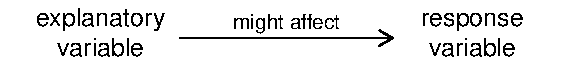
\includegraphics[scale=0.75]{figure/variables.pdf}
\end{figure}
\end{frame}

%---------------------------------------------
\begin{frame}
\large \textbf{Sampling Concepts}
\begin{itemize}
\item Samples and populations
\item Parameters and statistics
\item Statistical inference
\end{itemize}
\end{frame}

%---------------------------------------------
\begin{frame}{Sampling Concepts}
\begin{columns}
\column{0.6\textwidth}
\begin{itemize}
\item A \textbf{population} is the set of all individuals or cases of interest to the investigator. 
\item A \textbf{sample} is any subset selected from the population.
\end{itemize}
\column{0.4\textwidth}
\begin{figure}
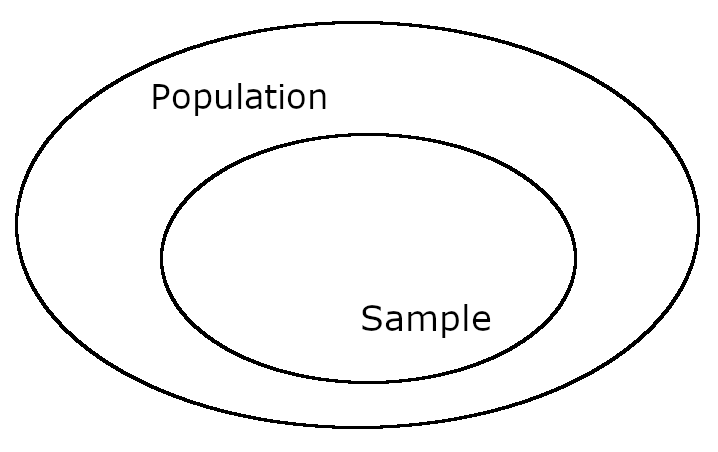
\includegraphics[scale=0.75]{figure/popsamp.png}
\end{figure}
\end{columns}
\vspace{10pt}
\emph{\underline{Example}}:\\
Population: All students that attend CSUEB.\\
Sample:  100 randomly selected CSUEB students. 
\end{frame}

%---------------------------------------------
\begin{frame}{Sampling Concepts}
\begin{itemize}
\item A \textbf{parameter} is a numerical characteristic of the population (fixed and usually unknown). 
\item A \textbf{statistic} is a numerical characteristic of the sample (varies depending on sample). \\
\end{itemize}
% \vspace{4.5cm}
\begin{figure}
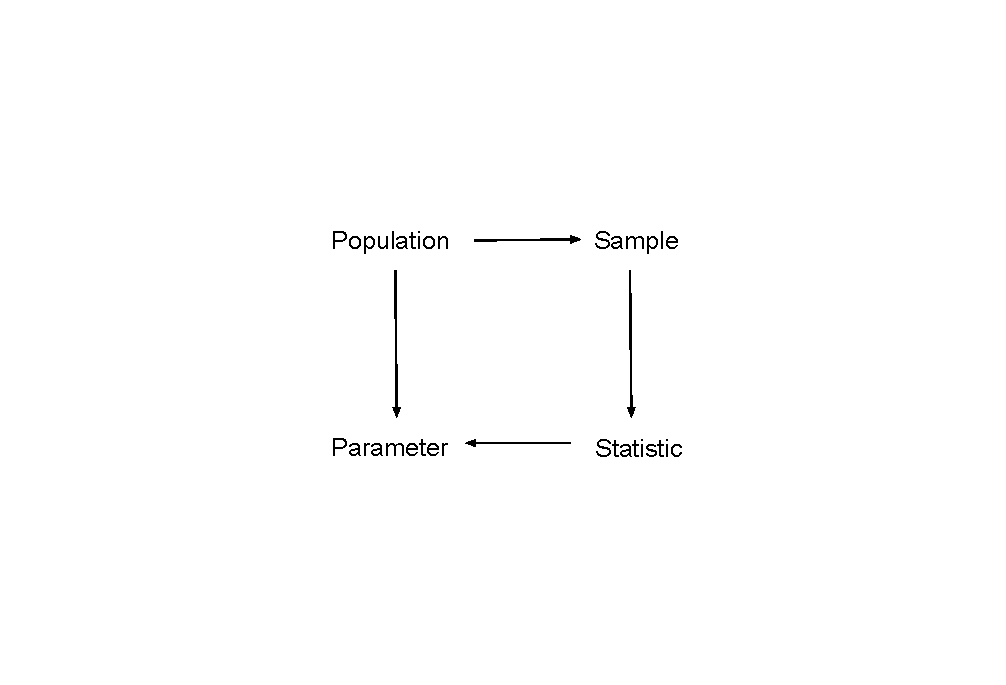
\includegraphics[scale=0.75]{figure/inference.pdf}
\end{figure}
\end{frame}

%---------------------------------------------
\begin{frame}{Sampling Concepts}
\emph{\underline{Example}}:\\ 
Parameter: Average height of all students that attend CSUEB.  This is a fixed number, but probably unknown since we might not have the time or resources to measure every student.\\
\vspace{10pt}
Statistic: Average height of 100 randomly selected CSUEB students.  Each sample will contain different individuals, and therefore yield a different value for the average height.\\
\end{frame}

%---------------------------------------------
\begin{frame}{Sampling Concepts}
Some notation for common parameters and statistics:\\
\vspace{10pt}

\begin{tabular}{|l|l|l|}
\hline
& parameter & statistic\\
\hline
mean & $\mu$ & $\bar{x}$\\
proportion & $p$ & $\hat{p}$\\
standard deviation & $\sigma$ & s\\
\hline
\end{tabular}
\end{frame}

%---------------------------------------------
\begin{frame}{Sampling Concepts}
\emph{\underline{Example}}: A Gallup poll\footnote{\tiny \url{https://news.gallup.com/poll/351035/public-backs-requiring-covid-vaccine-attend-school.aspx}}, conducted between May 18-23, 2021, asked the following question: 

\smallskip
Would you favor or oppose college students being required to receive a coronavirus/COVID-19 vaccine in order to attend classes in the fall?
\medskip

61\% of the respondents favored requiring vaccines for college students.  The results were based on web interviews of a random sample of 3,572 American adults who are members of the Gallup panel.  For this survey, describe the sample, population, statistic, and parameter.\\
\vspace{10pt}

{\color{blue}\emph{Solution:}}
\begin{enumerate}
{\color{blue}
\item Sample: 3,572 American adults
\item Population: all American adults
\item Statistics: 61\% favored requiring vaccines for college students
\item Parameter: proportion of all Americans that favored requiring vaccines for college students (during sampling period)}
\end{enumerate}
\end{frame}

%---------------------------------------------
\begin{frame}{Sampling Concepts}
\textbf{Statistical inference} is the process of using a random sample to infer properties about the greater population of interest.  A major task in statistical inference is to quantify the uncertainty of our estimates or predictions based on a random sample.  Mathematical or computational methods can be used to accomplish this task.\\
\vspace{15pt}

\emph{\underline{Example}}:  Going back to the Gallup poll, we are primarily interested in using the sample of respondents to make an inference about the proportion of all American adults that support requiring vaccines for college students.  The Gallup poll reported a \textbf{margin of error} of $\pm 2\%$, so we would expect the population proportion to be somewhere between 59\% and 63\%.  
\end{frame}

%---------------------------------------------
\begin{frame}
\large \textbf{Two primary types of data collection:}
\begin{itemize}
\item Observational studies
\item Experiments
\end{itemize}
\end{frame}

%---------------------------------------------
\begin{frame}{Observational Studies}
\begin{itemize}
\item \textbf{Observational study}: researcher collects data without interfering in the process that generates that data.  That is, data are gathered by monitoring what has occurred or by using historical records.
\vspace{5pt} 
\item Observational studies can be used to show \textbf{associations} between variables of interest, but generally do not support cause-and-effect relationships.
\vspace{5pt} 
\item \emph{\underline{Example}:} The Centers for Disease Control (CDC) uses telephone surveys to collect data on health-related risk behaviors. Respondents are asked questions about diet, exercise, smoking, and level of health care coverage.  
\end{itemize}
\end{frame}

%---------------------------------------------
\begin{frame}{Experimental Studies}
\begin{itemize}
\item \textbf{Experimental study}: researcher actively manipulates the explanatory variables and records their effect on the response variable.
\vspace{5pt}
\item For a \textbf{randomized experiment} individuals are randomly assigned to different treatment groups and the outcomes for the response variable are compared.
\vspace{5pt} 
\item Experiments can be used to infer \textbf{cause-and-effect} relationships between the response and explanatory variables.
\end{itemize}
\end{frame}

%---------------------------------------------
\begin{frame}{Experimental Studies: Example}
\begin{itemize}
\item Knee osteoarthritis (OA) is a common problem in the elderly population that results in pain and reduced quality of life.  
\vspace{5pt}
\item Researchers at Tufts Medical Center conducted a randomized experiment to evaluate the effectiveness of Tai Chi in treating OA symptoms.\footnote{\scriptsize Wang et al. (2009). ``Tai Chi is Effective in Treating Knee Osteoarthritis: A Randomized Controlled Trial." \url{https://www.ncbi.nlm.nih.gov/pmc/articles/PMC3023169/}}
\end{itemize}
\begin{figure}
\flushright
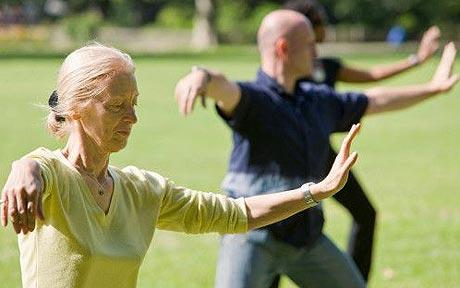
\includegraphics[scale=0.3]{figure/taiChi.jpg}
\end{figure}
\end{frame}
%Image from https://www.telegraph.co.uk/news/health/news/6453806/Tai-Chi-can-ease-the-pain-of-arthritis.html

%---------------------------------------------
\begin{frame}{Experimental Studies: Example}
\vspace{-2cm} 
\begin{itemize}
\item 40 patients with OA, aged 55 years and older, with no prior experience with Tai Chi, were recruited.
\vspace{5pt}
\item 20 patients were randomly assigned to 60-minute Tai Chi sessions twice-weekly for 12 weeks (\textbf{treatment group}).  The other 20 patients were assigned to 60 minute sessions on wellness education and stretching twice-weekly for 12 weeks (\textbf{control group}).
\vspace{5pt}
\item At the end of the 12 weeks, the patients in the Tai Chi group reported a significant decrease in knee pain when compared to the control group.
\end{itemize}
% Ask the class: What are some limitations of this study?
% Possible answer: Since respondents were recruited we don't know if the sample of adults was random and can be generalized.  It would also be good to replicate the study and experiment before making any strong conclusions.
\end{frame}



%---------------------------------------------
\begin{frame}{Experimental Studies: Example}
\begin{figure}
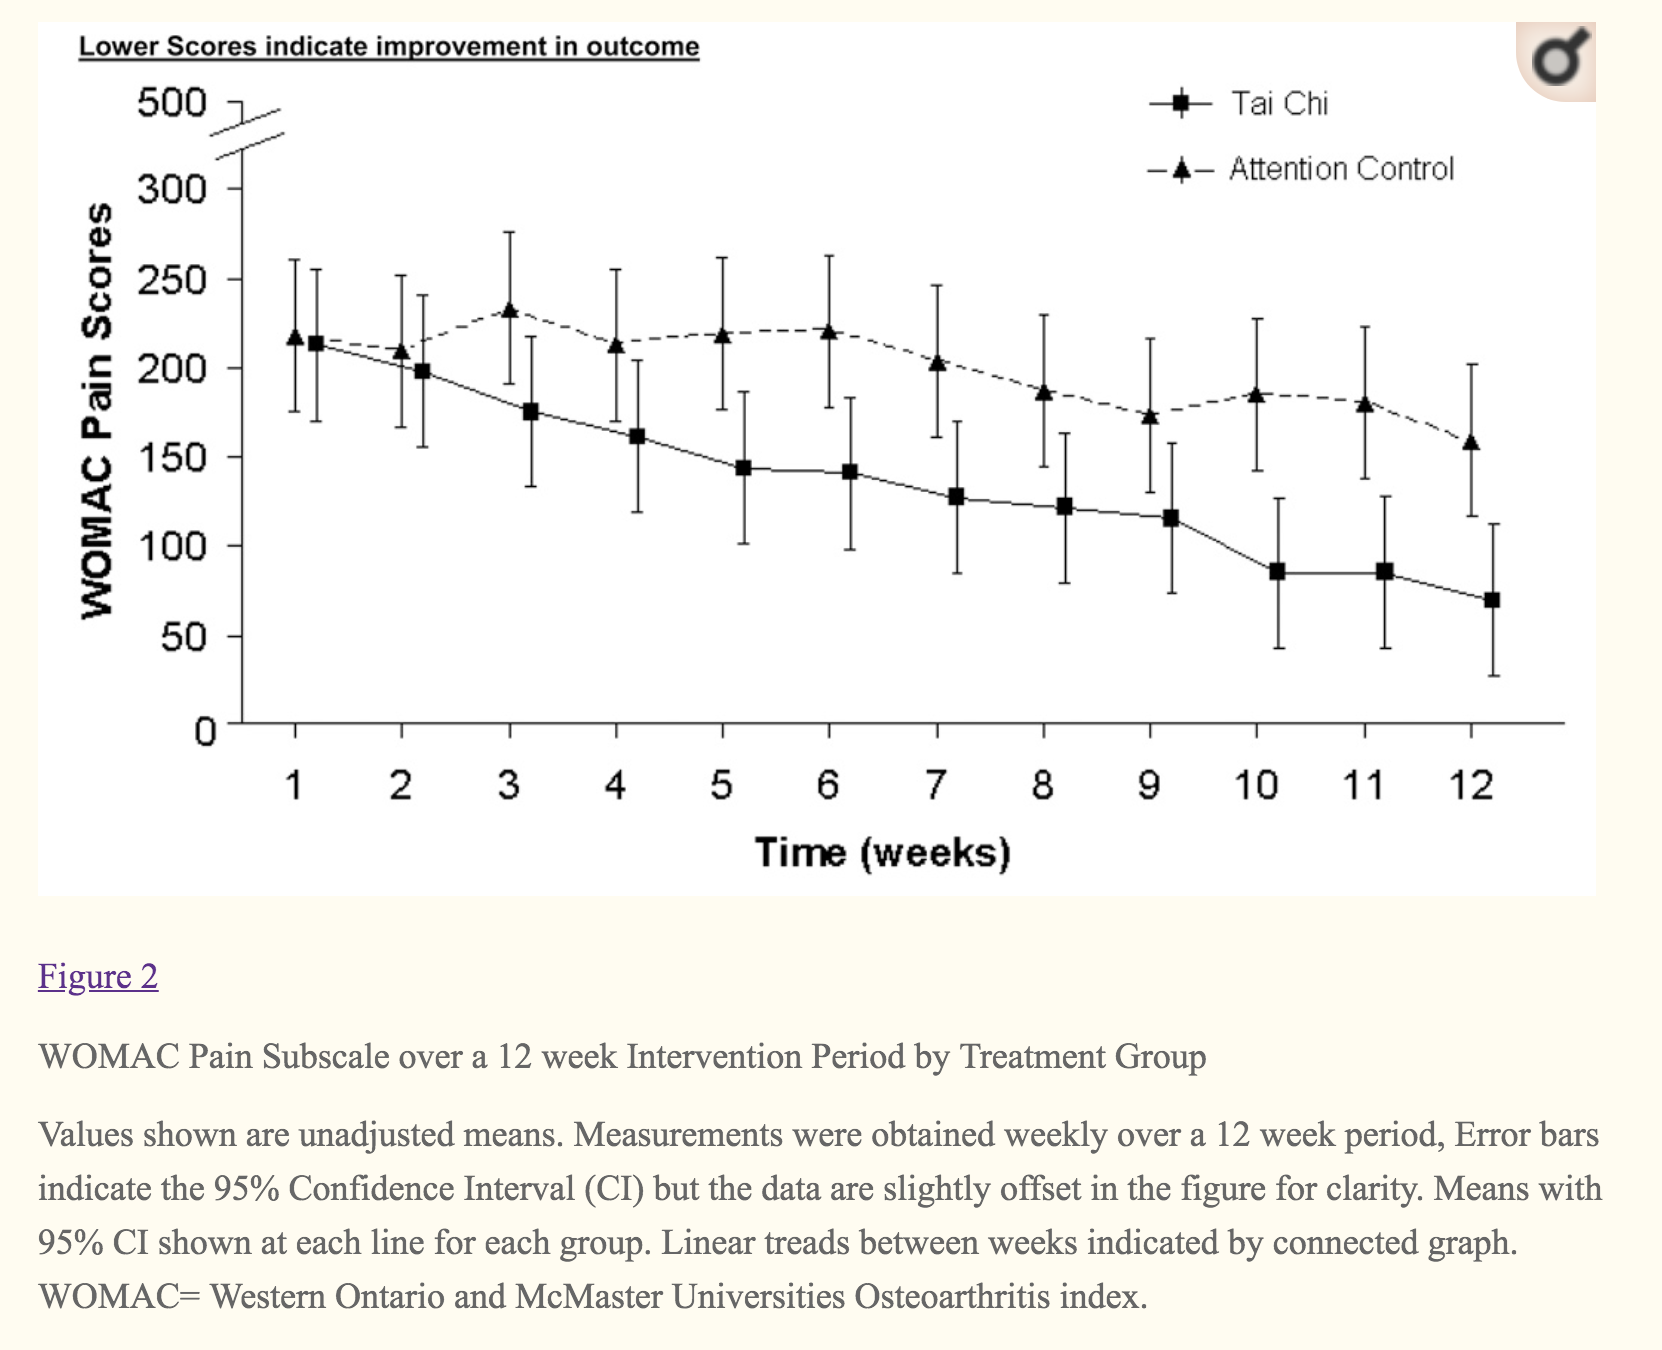
\includegraphics[scale=0.3]{figure/Pain12weeks.png}
\end{figure}
\end{frame}

%---------------------------------------------
\begin{frame}{Confounding Variables}
One reason it is difficult to establish causal relationships in observational studies is because of confounding variables. A \textbf{confounding variable} is a variable that is associated with both the response and explanatory variables, but is not accounted for by the researcher.
\end{frame}

%---------------------------------------------
\begin{frame}{Confounding Variables}
% \vspace{-3.5cm} 
\vspace{-1.75cm}
\emph{\underline{Example}}:  A researcher conducts an observational study by recording the number of hours of TV a sample of students watch and their GPAs.  The researcher finds that, in general, the more TV students watch, the lower their GPAs.  Does this necessarily mean that watching TV \emph{causes} students to have a lower GPA?  What are some examples of confounding variables?\\
\vspace{10pt}

{\color{blue} \emph{Solution:}\\
Since this is an observational study we cannot make cause-and-effect conclusions.  One confounding variable is the number of hours the students spend studying.}
\end{frame}

\end{document}